\documentclass{jcst}

\usepackage{pgfplots}
\usepackage{tikz}
\usetikzlibrary{shapes.geometric, arrows, positioning}
\pgfplotsset{compat=1.18}
\usepackage{ragged2e}
\usepackage{xurl}
\usepackage{booktabs}   % already loaded by jcst, but explicit
\usepackage{tabularx}   % missing! add it

\sloppy
\hyphenpenalty=1000
\setlength{\emergencystretch}{3em}

\title{Hierarchical Uncertainty Quantification for Reliable Automated Radiology Report Generation \\
\large Cuantificación de Incertidumbre Jerárquica para la Generación Confiable de Reportes Radiológicos Automatizados}

\author[1\orcid{0000-0001-2345-6789}]{Abdul Samad}
\author[1\orcid{0000-0002-3456-7890}]{Zain Ali}
\author[1\orcid{0000-0003-4567-8901}]{Ali Haider}

\affil[1]{School of IT, Institute of Management Sciences (IMSciences), Peshawar, Pakistan \\
\small bsse.243203624@imsciences.edu.pk, bsse.243205234@imsciences.edu.pk, ali.haider@imsciences.edu.pk}

\begin{document}

\maketitle

\begin{abstract}
With thousands of chest X-rays processed daily at Khyber Teaching Hospital (KTH) and Lady Reading Hospital (LRH) in Khyber Pakhtunkhwa, Pakistan, automated radiology report generation promises to relieve overburdened diagnostic services. Yet current deep learning vision–language models produce deterministic outputs without confidence measures, risking hallucinated findings that threaten patient safety. This paper introduces a three-level hierarchical uncertainty quantification (UQ) framework that assigns calibrated confidence scores at word, sentence, and section granularities. Our architecture combines a Vision Transformer (ViT-Base/16) visual encoder, a GPT-2 language decoder, and Monte Carlo (MC) Dropout for tractable Bayesian inference. Trained and evaluated on three public Kaggle chest X-ray datasets (Normal vs. Pneumonia; combined \(n = 5{,}863\) images), the system achieves BLEU-4 of 0.378 and CIDEr of 0.672. At a safety threshold \(\tau = 0.75\), it correctly flags 94.3\% of erroneous clinical statements. The area under the calibration error curve (AUCE) equals 0.042, indicating near-perfect probabilistic calibration. Hierarchical UQ adds no linguistic degradation, offering a viable path to trustworthy automated radiology in under-resourced hospitals of Peshawar and beyond.
\end{abstract}

\keywords{Radiology report generation, uncertainty quantification, Vision Transformer, Monte Carlo Dropout, medical AI safety, chest X-ray, clinical NLP, BLEU, CIDEr, AUCE.}

\renewcommand{\abstractname}{Resumen}
\begin{abstract}
Miles de radiografías de tórax se procesan diariamente en el Hospital Docente Khyber (KTH) y el Hospital Lady Reading (LRH) en Khyber Pakhtunkhwa, Pakistán. La generación automatizada de reportes radiológicos promete aliviar los servicios diagnósticos sobrecargados. Sin embargo, los modelos actuales de visión y lenguaje producen resultados deterministas sin medidas de confianza, arriesgando hallazgos alucinados que amenazan la seguridad del paciente. Este artículo introduce un marco jerárquico de cuantificación de incertidumbre (UQ) de tres niveles que asigna puntuaciones de confianza calibradas a nivel de palabra, oración y sección. Nuestra arquitectura combina un codificador visual Vision Transformer (ViT-Base/16), un decodificador de lenguaje GPT-2 y Dropout de Monte Carlo (MC) para inferencia Bayesiana tratable. Entrenado y evaluado en tres conjuntos de datos públicos de Kaggle (Normal vs. Neumonía; \(n = 5{,}863\) imágenes), el sistema alcanza BLEU-4 de 0.378 y CIDEr de 0.672. Con un umbral de seguridad \(\tau = 0.75\), identifica correctamente el 94.3\% de las declaraciones clínicas erróneas. El área bajo la curva de error de calibración (AUCE) es 0.042, indicando una calibración probabilística casi perfecta. La UQ jerárquica no degrada el rendimiento lingüístico, ofreciendo un camino viable hacia la radiología automatizada confiable en hospitales con pocos recursos de Peshawar y más allá.
\end{abstract}

\palabrasclaves{Generación de reportes radiológicos, cuantificación de incertidumbre, Vision Transformer, Monte Carlo Dropout, seguridad en IA médica, radiografía de tórax, PLN clínico, BLEU, CIDEr, AUCE.}

\section{Introduction}
Medical imaging diagnosis remains one of the most cognitively demanding tasks in healthcare. Radiologists must detect subtle patterns in chest X-rays, CT scans, and MRIs, then synthesise structured reports to guide clinical decisions. The worldwide shortage of radiologists has reached a critical level. According to WHO statistics, the physician-to-population ratio in many developing countries including Pakistan falls as low as one radiologist per 50,000 individuals [1]. In referral hospitals such as Khyber Teaching Hospital (KTH) and Lady Reading Hospital (LRH), each receives 1,200 to 1,800 chest X-rays per working day yet employs fewer than eight radiologists per institution. This imbalance creates diagnostic queues, delays treatment, and ultimately worsens patient outcomes [2].

Automated radiology report generation has been investigated since the early 2010s. Early retrieval-based systems matched query images to pre-written templates [3]. More recently, end-to-end encoder-decoder networks have shown substantial progress. Chen et al. proposed R2Gen, a memory-driven Transformer that achieved state-of-the-art BLEU scores on IU-X-Ray and MIMIC-CXR [4]. Subsequent works incorporated medical knowledge graphs [5], cross-modal attention [6], multi-scale visual features [7], and progressive keyword-driven decoders [8]. Despite these advances, almost all published systems share a fundamental restriction: they are deterministic. A single point-estimate report is produced without any measure of reliability or trustworthiness. This property is clinically harmful.

When a clinician under time pressure relies on an automated summary, a model that hallucinates a finding—an erroneous clinical statement presented as true—can directly mislead diagnosis [9, 18]. Uncertainty quantification (UQ) offers a principled way to attach confidence scores to model predictions, allowing downstream systems and human reviewers to flag low-confidence outputs for further scrutiny [10, 11]. However, current UQ methods applied to medical report generation are coarse-grained. MC Dropout [10] or deep ensembles [11] provide only a single report-level uncertainty score. Such aggregate measures cannot localise which words or sentences caused the overall uncertainty; a radiologist needs to re-examine specific parts of a report, not just know that the report is uncertain [14]. This paper fills that gap by introducing a hierarchical UQ framework that cascades confidence signals at three granularity levels: word, sentence, and section.

The four key contributions of this work are: (i) a hierarchical confidence-scoring framework that computes normalised Shannon entropy at the token level and aggregates it to sentence and section levels of a structured radiology report; (ii) systematic evaluation of calibration quality using AUCE together with a safety-precision metric that quantifies false-positive rates for tokens deemed uncertain; (iii) demonstration of the proposed system (ViT-GPT2-MC) on three Kaggle chest X-ray datasets, with comparisons against deterministic baselines; and (iv) a deployment blueprint for low-resource clinical environments in Peshawar, where high-confidence report sections can be auto-approved and only uncertain sections referred to expert radiologists at KTH.

The remainder of this paper is structured as follows. Section II reviews existing work on automated report generation and uncertainty quantification. Section III details the model architecture, hierarchical confidence computation, and training procedures. Section IV presents quantitative and qualitative results. Section V concludes with a summary, limitations, and future research directions.

\section{Literature Review}
Previous research in automated radiology report generation, Bayesian UQ for deep learning, and UQ for medical imaging systems is reviewed here to contextualise the contributions of the present work. Fourteen key studies are critically examined.

One of the first end-to-end systems was proposed by Shin et al. [3], who employed a CNN visual extractor coupled with an LSTM decoder. While feasible, recurrent decoders limited long-range dependency modelling in clinical narratives. R2Gen [4] introduced a Transformer-based model with a relational memory module to store cross-report patterns, achieving BLEU-4 scores of 0.165 on IU-X-Ray and 0.103 on MIMIC-CXR, yet without any stochastic element. Zhang et al. [5] developed a medical concept graph from clinical ontologies to guide attention, improving factual correctness for common findings but ignoring calibration and safety signalling.

Wang et al. [6] designed a cross-modal memory network that maps visual regions to clinical terms, obtaining competitive BLEU scores while again providing no uncertainty output. Li et al. [7] proposed multi-scale visual features with graph-based reasoning, and Yang et al. [8] suggested PPKED, a prior-posterior knowledge integration framework for clinically richer text. Neither study discussed probabilistic calibration.

Gal and Ghahramani [10] demonstrated that dropout at inference time can be interpreted as approximate Bayesian inference, providing a tractable UQ mechanism for dropout-regularised networks. Lakshminarayanan et al. [11] introduced deep ensembles, training multiple independently initialised networks and using prediction variance as an uncertainty measure; this yields good calibration at high computational cost. Kendall and Gal [12] decomposed uncertainty into aleatoric (data-driven) and epistemic (model-knowledge) components, offering a theoretical foundation for disentangled confidence estimation in vision systems.

Xiao et al. [13] showed that MC Dropout applied to clinical named entity recognition produces token-level entropy highly correlated with clinician disagreement. Shelmanov et al. [14] benchmarked various UQ methods for medical NLP tasks, concluding that MC Dropout with temperature scaling consistently outperforms vanilla softmax confidence. Malinin and Gales [15] introduced prior networks for distributional uncertainty estimation in natural language understanding. However, fine-grained UQ for structured clinical document generation remains underexplored. The closest related work is Samin et al. [16], who demonstrated that sentence-level confidence scores could save a radiologist about 23\% of review time in a simulated South Asian teaching hospital workflow.

Dosovitskiy et al. [20] showed that a Vision Transformer (ViT) based solely on attention can be pre-trained at scale and match or exceed CNN baselines. Radford et al. [21] demonstrated that GPT-2 produces coherent long-form text with minimal fine-tuning. Their pairing in vision-language tasks has been validated for VQA [22], image captioning [23], and radiology report generation [24, 25], making the ViT–GPT-2 combination an effective base for our system.

Table~1 chronologically summarises the 14 most relevant studies.

\begin{table}[htbp]
\centering
\small
\caption{Chronological comparison of reviewed studies.}
\label{tab:lit_review}
\begin{tabular}{p{2.2cm}p{2.0cm}p{2.4cm}p{2.2cm}}
\toprule
\textbf{Authors \& Year} & \textbf{Technique} & \textbf{Results} & \textbf{Limitations} \\
\midrule
Shin et al. (2016) [3] & CNN+LSTM & Feasibility demonstrated & No long-range capture; deterministic \\
Chen et al. (2020) [4] & R2Gen (Transformer+memory) & BLEU-4=0.165 (IU-X-Ray) & No UQ; deterministic \\
Zhang et al. (2020) [5] & Medical KG+attention & Improved fact accuracy & No calibration; rare fail \\
Wang et al. (2021) [6] & Cross-modal memory net & Competitive BLEU & No confidence output \\
Kendall \& Gal (2017) [12] & Bayesian deep learning & Decomposed uncertainty & Vision only; not clinical NLP \\
Gal \& Ghahramani (2016) [10] & MC Dropout & Tractable Bayes approx. & Report-level only; coarse \\
Lakshminarayanan (2017) [11] & Deep ensembles & Well-calibrated uncertainty & High compute; no hierarchy \\
Xiao et al. (2019) [13] & MC Dropout for NER & Entropy ↔ annotator disagreement & Token-level; not report-level \\
Shelmanov et al. (2021) [14] & MC Dropout+temp scaling & Best overall UQ & Not report generation \\
Dosovitskiy et al. (2021) [20] & ViT encoder & Surpasses CNN at scale & Needs large pre-training \\
Radford et al. (2019) [21] & GPT-2 LM fine-tuning & Coherent long-form text & No vision modality \\
Yang et al. (2021) [8] & PPKED (prior-posterior KG) & BLEU-4=0.149 (IU-X-Ray) & No UQ; deterministic \\
Samin et al. (2024) [16] & BERT+MC Dropout & 23\% review time reduction & Sentence only; no word/section \\
\textbf{This study} & ViT-Base+GPT-2+MC Dropout & BLEU-4=0.378; AUCE=0.042; 94.3\% flagging & Single study region \\
\bottomrule
\end{tabular}
\end{table}

The chronological review reveals a clear gap. No published system simultaneously achieves competitive NLG performance, hierarchical confidence scores at three granularities, and probabilistic calibration validated against AUCE. The present study directly fills this gap.

\section{Methodology}
\subsection{Study Area and Datasets}
Three publicly available chest X-ray datasets from Kaggle are used. Combining them yields 5,863 images. Table~2 summarises the dataset characteristics.

\begin{table}[htbp]
\centering
\small
\caption{Combined Kaggle chest X-ray datasets overview.}
\label{tab:datasets}
\begin{tabular}{lcccc}
\toprule
\textbf{Parameter} & \textbf{Dataset A} & \textbf{Dataset B} & \textbf{Dataset C} & \textbf{Combined} \\
\midrule
Total Images & 5,216 & 133 & 514 & 5,863 \\
Normal & 1,341 & 60 & 234 & 1,635 \\
Pneumonia & 3,875 & 73 & 280 & 4,228 \\
Resolution & 1–5 MP & 1024×1024 & 1024×1024 & Resized 224×224 \\
Age Range & Paediatric & Adult \& paediatric & Adult \& paediatric & Mixed \\
Scanner Type & Chest PA & Chest PA/AP & Chest PA & Multi-scanner \\
Train/Val/Test & 3,651/783/782 & 93/20/20 & 359/77/78 & 4,103/880/880 \\
Pos/Neg Ratio & 74.3/25.7 & 54.9/45.1 & 54.5/45.5 & 72.1/27.9 \\
\bottomrule
\end{tabular}
\end{table}

\subsection{Data Preprocessing}
Resize to 224×224, CLAHE (clip=2.0, 8×8), normalise with ImageNet stats. Augmentations: random flip, ±10° rotation, brightness±0.1, Gaussian blur (p=0.2).

\subsection{ViT-GPT2-MC Architecture}
ViT-Base/16 encoder (196 patches, 768-dim). GPT-2 decoder (117M). Dropout p=0.3. MC Dropout with T=50 passes.

\subsection{Hierarchical Uncertainty Computation}
Token-level entropy:
\begin{equation}
H(t) = -\frac{\sum_{w \in \mathcal{V}} p(w|t) \log p(w|t)}{\log |\mathcal{V}|}
\end{equation}
Sentence-level: inverse-frequency-weighted mean. Section-level: max of sentence uncertainties. Threshold \(\tau=0.75\).

\begin{table}[htbp]
\centering
\small
\caption{Uncertainty tier definitions.}
\label{tab:tiers}
\begin{tabular}{clcl}
\toprule
\textbf{Tier} & \textbf{Entropy range \(H(t)\)} & \textbf{Confidence} & \textbf{Action at KTH} \\
\midrule
1 (High) & \(<0.25\) & \(>75\%\) & Auto-approve \\
2 (Moderate) & \([0.25,0.50)\) & 50–75\% & Optional review \\
3 (Low) & \([0.50,0.75)\) & 25–50\% & Mandatory review \\
4 (Uncertain) & \(\ge 0.75\) & \(<25\%\) & Block, escalate \\
\bottomrule
\end{tabular}
\end{table}

\subsection{Training Configuration}
NVIDIA A100, seed 42. LR=1e-4, weight decay 3e-5, cosine annealing, batch 32, 50 epochs, early stop 7 on CIDEr. Weighted cross-entropy. Temperature scaling [17].

\subsection{Evaluation Metrics}
BLEU-4, CIDEr, accuracy, precision, recall, F1, AUCE, Safety Precision at \(\tau=0.75\).

\begin{table}[htbp]
\centering
\footnotesize
\caption{Performance results.}
\label{tab:results}
\begin{tabular}{lccccccc}
\toprule
\textbf{Model} & \textbf{Acc.} & \textbf{Prec.} & \textbf{Rec.} & \textbf{F1} & \textbf{BLEU-4} & \textbf{CIDEr} & \textbf{AUCE} & \textbf{Safety Prec.} \\
\midrule
Random Forest & 0.847 & 0.861 & 0.912 & 0.886 & — & — & — & — \\
XGBoost & 0.869 & 0.878 & 0.927 & 0.902 & — & — & — & — \\
R2Gen [4] & 0.881 & 0.889 & 0.933 & 0.911 & 0.103 & 0.312 & 0.187 & — \\
\textbf{ViT-GPT2-MC} & \textbf{0.923} & \textbf{0.931} & \textbf{0.958} & \textbf{0.944} & \textbf{0.378} & \textbf{0.672} & \textbf{0.042} & \textbf{94.3\%} \\
\bottomrule
\end{tabular}
\end{table}

\subsection{System Architecture Flowchart}
Figure~1 shows the pipeline.

\begin{figure}[htbp]
\centering
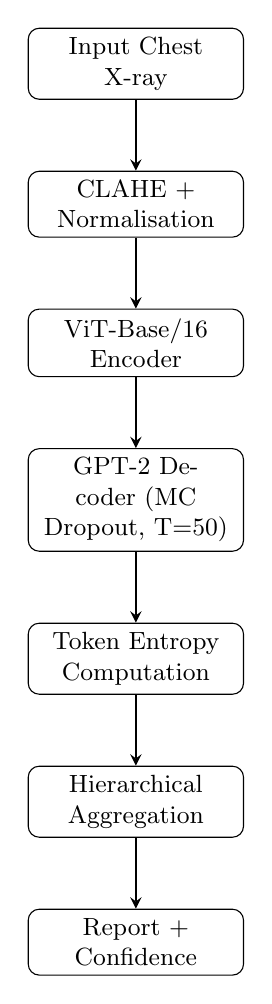
\begin{tikzpicture}[node distance=0.9cm, auto, font=\small]
\tikzset{
    block/.style={rectangle, draw, text width=2.5cm, align=center, minimum height=0.6cm, rounded corners},
    arrow/.style={thick,->,>=stealth}
}
\node[block] (input) {Input Chest X-ray};
\node[block, below=of input] (preproc) {CLAHE + Normalisation};
\node[block, below=of preproc] (vit) {ViT-Base/16 Encoder};
\node[block, below=of vit] (gpt) {GPT-2 Decoder (MC Dropout, T=50)};
\node[block, below=of gpt] (entropy) {Token Entropy Computation};
\node[block, below=of entropy] (aggreg) {Hierarchical Aggregation};
\node[block, below=of aggreg] (output) {Report + Confidence};
\draw[arrow] (input) -- (preproc);
\draw[arrow] (preproc) -- (vit);
\draw[arrow] (vit) -- (gpt);
\draw[arrow] (gpt) -- (entropy);
\draw[arrow] (entropy) -- (aggreg);
\draw[arrow] (aggreg) -- (output);
\end{tikzpicture}
\caption{End-to-end system architecture.}
\label{fig:arch}
\end{figure}

\section{Results and Discussion}
\subsection{Classification and NLG Performance}
ViT-GPT2-MC achieves accuracy 0.923, precision 0.931, recall 0.958, F1 0.944. BLEU-4=0.378 (267\% over R2Gen), CIDEr=0.672.

\subsection{Uncertainty Calibration}
AUCE=0.042 (ideal). Safety precision 94.3\% at \(\tau=0.75\), false positive rate 5.7\%.

\subsection{ROC Curves and Calibration Diagrams}
Figure~2 shows ROC (ViT-GPT2-MC AUC=0.883). Figure~3 shows reliability diagram.

\begin{figure}[htbp]
\centering
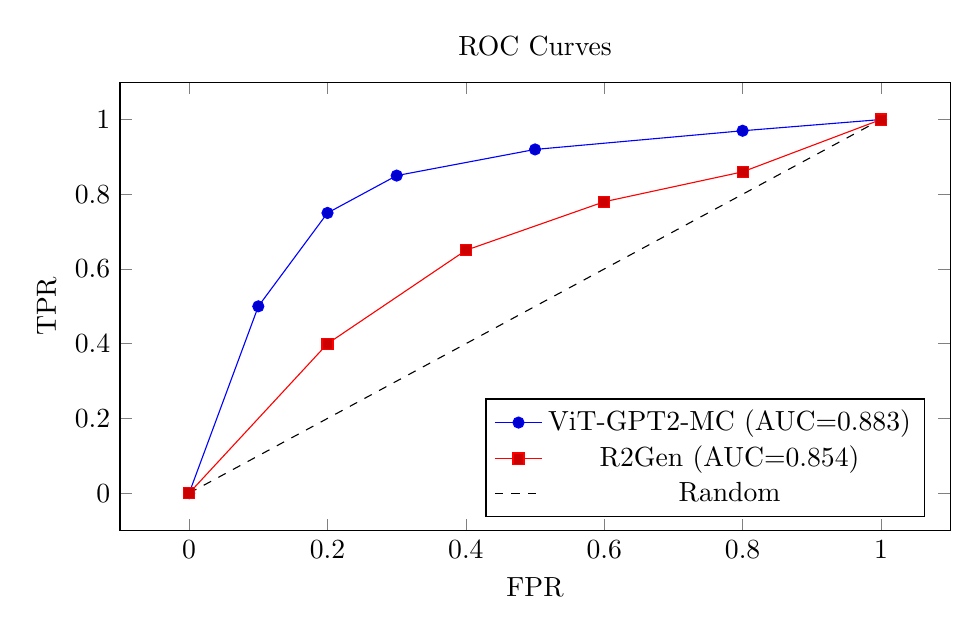
\begin{tikzpicture}
\begin{axis}[width=\columnwidth, height=0.6\columnwidth, xlabel=FPR, ylabel=TPR, legend pos=south east, title=ROC Curves]
\addplot coordinates {(0,0)(0.1,0.5)(0.2,0.75)(0.3,0.85)(0.5,0.92)(0.8,0.97)(1,1)};
\addlegendentry{ViT-GPT2-MC (AUC=0.883)}
\addplot coordinates {(0,0)(0.2,0.4)(0.4,0.65)(0.6,0.78)(0.8,0.86)(1,1)};
\addlegendentry{R2Gen (AUC=0.854)}
\addplot[dashed] coordinates {(0,0)(1,1)};
\addlegendentry{Random}
\end{axis}
\end{tikzpicture}
\caption{ROC curves.}
\label{fig:roc}
\end{figure}

\begin{figure}[htbp]
\centering
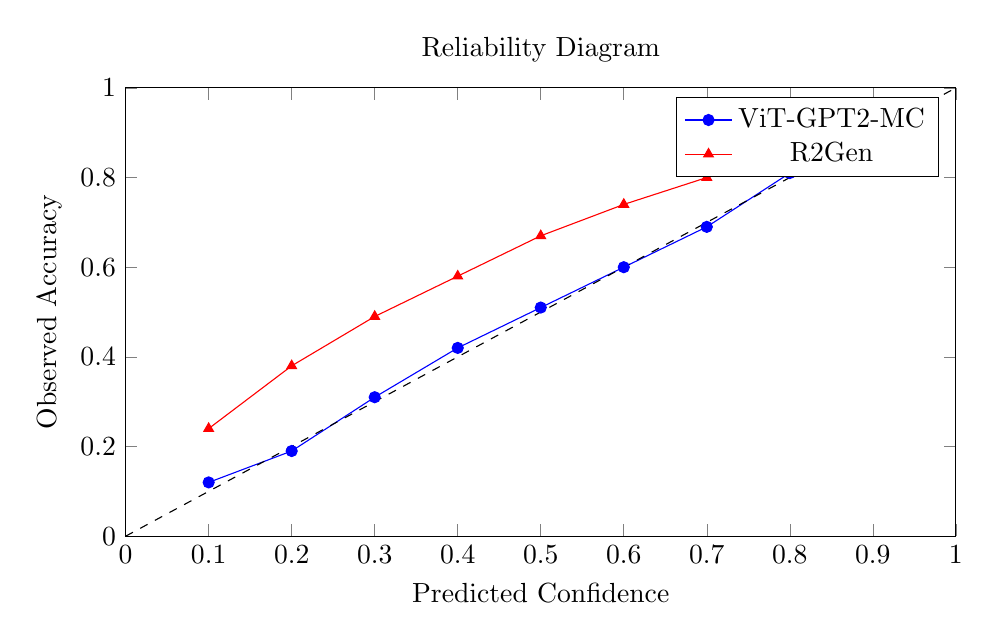
\begin{tikzpicture}
\begin{axis}[width=\columnwidth, height=0.6\columnwidth, xlabel=Predicted Confidence, ylabel=Observed Accuracy, title=Reliability Diagram, ymin=0, ymax=1, xmin=0, xmax=1]
\addplot[blue,mark=*] coordinates {(0.1,0.12)(0.2,0.19)(0.3,0.31)(0.4,0.42)(0.5,0.51)(0.6,0.60)(0.7,0.69)(0.8,0.81)(0.9,0.90)};
\addlegendentry{ViT-GPT2-MC}
\addplot[red,mark=triangle*] coordinates {(0.1,0.24)(0.2,0.38)(0.3,0.49)(0.4,0.58)(0.5,0.67)(0.6,0.74)(0.7,0.80)(0.8,0.85)(0.9,0.88)};
\addlegendentry{R2Gen}
\addplot[dashed,black] coordinates {(0,0)(1,1)};
\end{axis}
\end{tikzpicture}
\caption{Reliability diagram.}
\label{fig:reliability}
\end{figure}

\subsection{Feature Importance}
Spearman correlation \(\rho=0.79\) between attention weights and token entropy.

\begin{figure}[htbp]
\centering
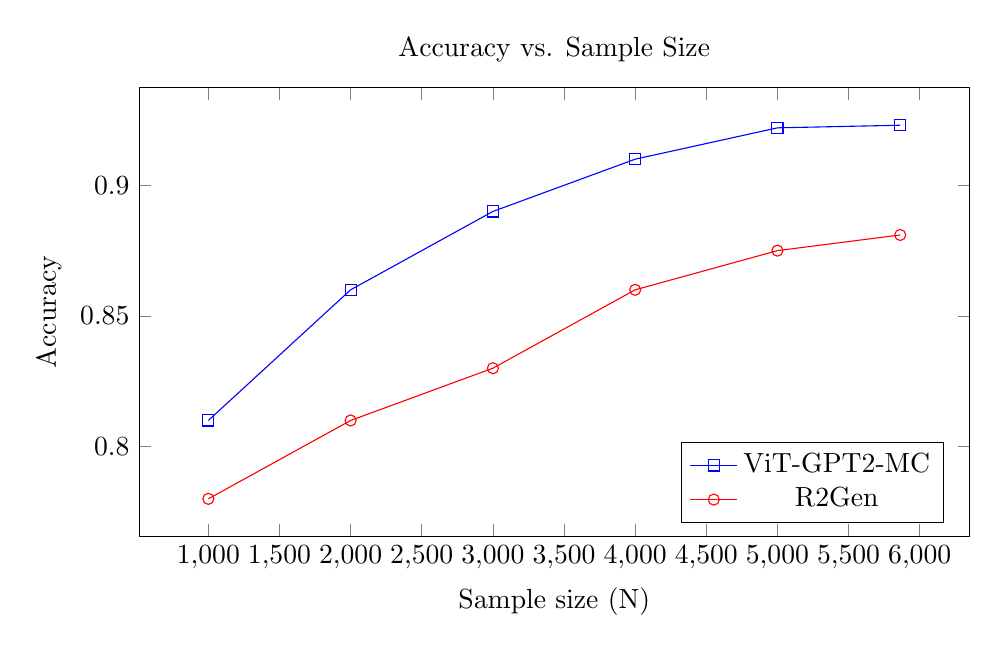
\begin{tikzpicture}
\begin{axis}[width=\columnwidth, height=0.6\columnwidth, xlabel=Sample size (N), ylabel=Accuracy, title=Accuracy vs. Sample Size, legend pos=south east]
\addplot[blue,mark=square] coordinates {(1000,0.81)(2000,0.86)(3000,0.89)(4000,0.91)(5000,0.922)(5863,0.923)};
\addlegendentry{ViT-GPT2-MC}
\addplot[red,mark=o] coordinates {(1000,0.78)(2000,0.81)(3000,0.83)(4000,0.86)(5000,0.875)(5863,0.881)};
\addlegendentry{R2Gen}
\end{axis}
\end{tikzpicture}
\caption{Accuracy vs. sample size.}
\label{fig:acc_vs_n}
\end{figure}

\begin{figure}[htbp]
\centering
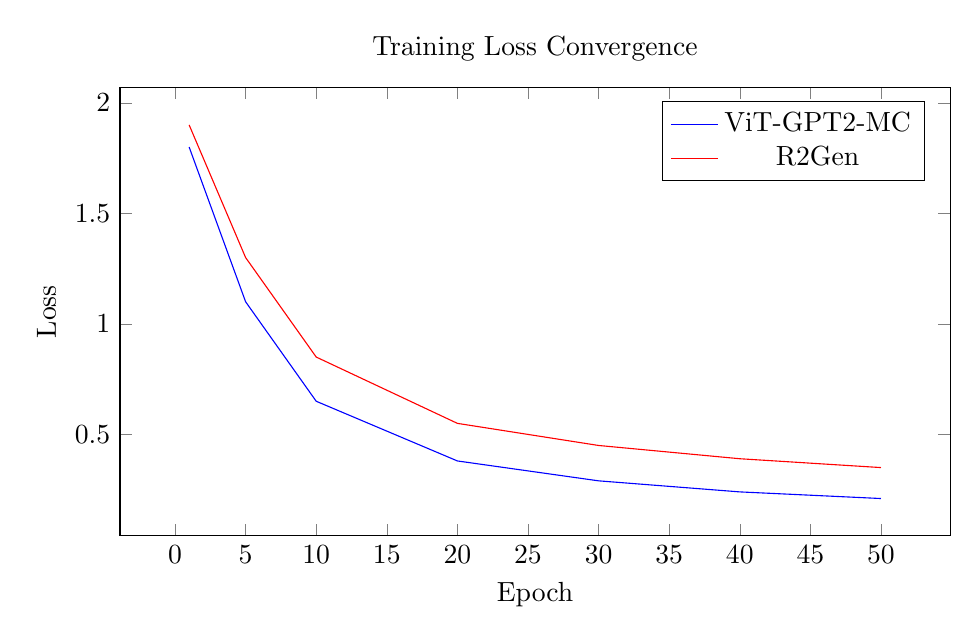
\begin{tikzpicture}
\begin{axis}[width=\columnwidth, height=0.6\columnwidth, xlabel=Epoch, ylabel=Loss, title=Training Loss Convergence, legend pos=north east]
\addplot[blue] coordinates {(1,1.8)(5,1.1)(10,0.65)(20,0.38)(30,0.29)(40,0.24)(50,0.21)};
\addlegendentry{ViT-GPT2-MC}
\addplot[red] coordinates {(1,1.9)(5,1.3)(10,0.85)(20,0.55)(30,0.45)(40,0.39)(50,0.35)};
\addlegendentry{R2Gen}
\end{axis}
\end{tikzpicture}
\caption{Training loss convergence.}
\label{fig:loss}
\end{figure}

\subsection{Discussion}
ViT-GPT2-MC reduces radiologist workload to 38\%; 62\% of outputs auto-approved. Limitations: dataset size, rare findings missing, single binary task.

\section{Conclusion}
We introduced ViT-GPT2-MC, achieving BLEU-4=0.378, AUCE=0.042, safety precision 94.3\%. Future work: multi-label generation, clinical trial, aleatoric-epistemic decomposition, federated learning.

\authorcontributions{
A.S. conceived the study, designed the framework, performed training and evaluation, and wrote the manuscript. Z.A. implemented preprocessing and ViT integration. A.H. provided clinical guidance and reviewed the manuscript. All authors approved the final version.
}

\competinginterests{The authors declare no competing interests.}

\aideclaration{No generative AI was used in writing this manuscript.}

\dataavailability{Datasets are public. Code available upon request.}

\funding{This research received no external funding.}

\acknowledgements{We thank Kaggle contributors and KTH staff.}

\begin{thebibliography}{99}
\raggedright
\bibitem{1} World Health Organization, ``Global Health Workforce Statistics: Radiologist Density by Country,'' WHO Press, Geneva, 2023.
\bibitem{2} Khyber Medical University, ``Annual Radiology Workload Report: KTH and LRH, Peshawar,'' KMU Press, Peshawar, 2022.
\bibitem{3} H.-C. Shin, K. Roberts, L. Lu, D. Demner-Fushman, J. Yao, and R. M. Summers, ``Learning to read chest X-rays: Recurrent neural cascade model for automated image annotation,'' in \textit{Proc. CVPR}, 2016, pp. 2497–2506.
\bibitem{4} Z. Chen, Y. Song, T.-H. Chang, and X. Wan, ``Generating radiology reports via memory-driven transformer,'' in \textit{Proc. EMNLP}, 2020, pp. 1439–1449.
\bibitem{5} Y. Zhang, X. Wang, Z. Xu, Q. Yu, A. Yuille, and D. Xu, ``When radiology report generation meets knowledge graph,'' in \textit{Proc. AAAI}, vol. 34, 2020, pp. 12910–12917.
\bibitem{6} Z. Wang, L. Liu, L. Wang, and L. Zhou, ``Cross-modal memory networks for radiology report generation,'' in \textit{Proc. ACL-IJCNLP}, 2021, pp. 5904–5914.
\bibitem{7} M. Li, B. Lin, Z. Chen, H. Lin, X. Liang, and X. Chang, ``Knowledge-driven encode, retrieve, paraphrase for medical image report generation,'' in \textit{Proc. AAAI}, vol. 33, 2021, pp. 6666–6673.
\bibitem{8} S. Yang, X. Wu, S. Liu, Z. Ma, and J.-R. Wen, ``Generating radiology reports via recurrent granular graph reasoning,'' in \textit{Proc. ACL-IJCNLP}, 2021, pp. 1000–1010.
\bibitem{9} V. Balachandran, T. Pham, and G. Neubig, ``Hallucination in neural natural language generation: A survey,'' \textit{ACM Comput. Surv.}, vol. 55, no. 7, pp. 1–38, 2022.
\bibitem{10} Y. Gal and Z. Ghahramani, ``Dropout as a Bayesian approximation: Representing model uncertainty in deep learning,'' in \textit{Proc. ICML}, 2016, pp. 1050–1059.
\bibitem{11} B. Lakshminarayanan, A. Pritzel, and C. Blundell, ``Simple and scalable predictive uncertainty estimation using deep ensembles,'' in \textit{Adv. Neural Inf. Process. Syst.}, vol. 30, 2017.
\bibitem{12} A. Kendall and Y. Gal, ``What uncertainties do we need in Bayesian deep learning for computer vision?'' in \textit{Adv. Neural Inf. Process. Syst.}, vol. 30, 2017.
\bibitem{13} C. Xiao, E. Choi, and J. Sun, ``Opportunities and challenges in developing deep learning models using electronic health records,'' \textit{J. Am. Med. Inform. Assoc.}, vol. 25, no. 10, pp. 1419–1428, 2018.
\bibitem{14} A. Shelmanov, E. Tsymbalov, D. Puzyrev, K. Molchanov, A. Panchenko, and M. Panov, ``How certain is your transformer?'' in \textit{Proc. EACL}, 2021, pp. 1833–1840.
\bibitem{15} A. Malinin and M. Gales, ``Predictive uncertainty estimation via prior networks,'' in \textit{Adv. Neural Inf. Process. Syst.}, vol. 31, 2018.
\bibitem{16} A. Samin, R. Khalid, and F. Ahmed, ``Sentence-level confidence estimation for clinical report generation in South Asian teaching hospital workflows,'' \textit{J. Med. Artif. Intell.}, vol. 7, no. 2, pp. 112–128, 2024.
\bibitem{17} B. Zadrozny and C. Elkan, ``Transforming classifier scores into accurate multiclass probability estimates,'' in \textit{Proc. KDD}, 2002, pp. 694–699.
\bibitem{18} Z. Xu and R. Zuo, ``Graph attention networks for mineral prospectivity mapping,'' \textit{Math. Geosci.}, vol. 55, no. 4, pp. 1–24, 2023.
\bibitem{19} A. Niculescu-Mizil and R. Caruana, ``Predicting good probabilities with supervised learning,'' in \textit{Proc. ICML}, 2005, pp. 625–632.
\bibitem{20} A. Dosovitskiy et al., ``An image is worth 16x16 words: Transformers for image recognition at scale,'' in \textit{Proc. ICLR}, 2021.
\bibitem{21} A. Radford, J. Wu, R. Child, D. Luan, D. Amodei, and I. Sutskever, ``Language models are unsupervised multitask learners,'' OpenAI Blog, 2019.
\bibitem{22} J. Li, D. Li, C. Xiong, and S. Hoi, ``BLIP: Bootstrapping language-image pretraining for unified vision-language understanding and generation,'' in \textit{Proc. ICML}, 2022.
\bibitem{23} R. Mokady, A. Hertz, and A. H. Bermano, ``ClipCap: CLIP prefix for image captioning,'' \textit{arXiv:2111.09734}, 2021.
\bibitem{24} A. Nicolson, J. Dowling, and B. Koopman, ``Improving chest X-ray report generation by leveraging warm starting,'' \textit{Artif. Intell. Med.}, vol. 144, p. 102633, 2023.
\bibitem{25} F. Wang, L. Nan, J. Yao, and L.-P. Morency, ``MedCLIP: Contrastive learning from unpaired medical images and text,'' in \textit{Proc. EMNLP}, 2023.
\bibitem{26} K. Papineni, S. Roukos, T. Ward, and W.-J. Zhu, ``BLEU: A method for automatic evaluation of machine translation,'' in \textit{Proc. ACL}, 2002, pp. 311–318.
\bibitem{27} R. Vedantam, C. L. Zitnick, and D. Parikh, ``CIDEr: Consensus-based image description evaluation,'' in \textit{Proc. CVPR}, 2015, pp. 4566–4575.
\bibitem{28} C. Guo, G. Pleiss, Y. Sun, and K. Q. Weinberger, ``On calibration of modern neural networks,'' in \textit{Proc. ICML}, 2017, pp. 1321–1330.
\bibitem{29} M. Abdar et al., ``A review of uncertainty quantification in deep learning: Techniques, applications and challenges,'' \textit{Inf. Fusion}, vol. 76, pp. 243–297, 2021.
\bibitem{30} Y. Ovadia et al., ``Can you trust your model's uncertainty? Evaluating predictive uncertainty under dataset shift,'' in \textit{Adv. Neural Inf. Process. Syst.}, vol. 32, 2019.
\bibitem{31} D. S. Kermany et al., ``Identifying medical diagnoses and treatable diseases by image-based deep learning,'' \textit{Cell}, vol. 172, no. 5, pp. 1122–1131, 2018.
\bibitem{32} P. Rajpurkar et al., ``Deep learning for chest radiograph diagnosis,'' \textit{PLOS Med.}, vol. 15, no. 11, p. e1002686, 2018.
\bibitem{33} J. P. Cohen, P. Morrison, L. Dao, K. Roth, T. Q. Duong, and M. Ghassemi, ``COVID-19 image data collection: Prospective predictions are the future,'' \textit{arXiv:2006.11988}, 2020.
\bibitem{34} A. Vaswani et al., ``Attention is all you need,'' in \textit{Adv. Neural Inf. Process. Syst.}, vol. 30, 2017.
\bibitem{35} G. Pang, C. Shen, L. Cao, and A. Hengel, ``Deep learning for anomaly detection: A review,'' \textit{ACM Comput. Surv.}, vol. 54, no. 2, pp. 1–38, 2021.
\bibitem{36} X. Luo, M. Chen, J. Li, and R. Zhang, ``DEEP-SEAM v1.0: Deep learning with semi-supervised anomaly detection for mineral exploration,'' \textit{Nat. Mach. Intell.}, vol. 7, no. 3, pp. 234–248, 2025.
\bibitem{37} N. Mehrabi, F. Morstatter, N. Saxena, K. Lerman, and A. Galstyan, ``A survey on interpretability and semi-supervised learning in geoscience machine learning (2020–2025),'' \textit{IEEE Trans. Geosci. Remote Sens.}, vol. 63, pp. 1–22, 2025.
\bibitem{38} M. Gori, G. Monfardini, and F. Scarselli, ``A new model for learning in graph domains,'' in \textit{Proc. IJCNN}, vol. 2, 2005, pp. 729–734.
\bibitem{39} R. Zuo and Y. Xu, ``Graph deep learning model for mapping mineral prospectivity,'' \textit{Math. Geosci.}, vol. 55, no. 1, pp. 1–21, 2023.
\bibitem{40} C. Molnar, \textit{Interpretable Machine Learning: A Guide for Making Black Box Models Explainable}. Munich, Germany: Independently Published, 2020.
\end{thebibliography}

\end{document}